\section{Observation-window sensitivity check}\label{app:window_check}

The network-estimation check reported in the main text (Section~\ref{sec:res_network_check})
treated the slow context as static, cross-sectional heterogeneity: for a given level of
within-group variation, $SD_P$, each simulated person's context value $P_i$ was drawn
independently from $\mathcal N(\mu_P, SD_P)$. This section asks a related but distinct
question: rather than varying the amount of context heterogeneity directly, how does the
same omitted-context bias depend on how long observations are aggregated relative to the
timescale over which the context itself fluctuates? This is the dynamic generalization of
the equivalence argument in Kruis and Maris (2016) and Marsman et al. (2018): the same
identification problem, expressed through the observation timescale rather than through an
arbitrary heterogeneity parameter.

We generated each simulated person's context value as the time-average of an
Ornstein-Uhlenbeck process,
\[
dP = -\kappa(P - \mu_P)\,dt + \sigma_P\,dW,
\]
with $\kappa = 0.20$ (matching the main model's calibrated mean-reversion rate, so the
resulting autocorrelation time $\tau_P = 1/\kappa$ has the same meaning as elsewhere in the
paper) and $\sigma_P$ chosen so the process's stationary standard deviation matched the
largest condition examined in the main check ($SD_P = 1.0$). Symptom generation and network
estimation followed the same pairwise model and nodewise logistic-regression estimator as
the main check (Section~\ref{sec:network_estimation_check}), using each person's
window-averaged context, $\bar P_W = \tfrac{1}{W}\sum_{t=1}^W P(t)$, in place of a
directly-drawn $P_i$. We varied the observation window $W$ (in simulation steps) from
$W/\tau_P \approx 0.004$ (approximately instantaneous, comparable to a single cross-sectional
measurement) to $W/\tau_P = 20$ (aggregation over twenty times the context's own
autocorrelation time), averaged over 6 independently drawn data-generating networks and 8
replicates per network.

Figure~\ref{fig:network_window_check} summarizes the results. As expected from the
Ornstein-Uhlenbeck process's known time-averaging behavior, the effective between-person
standard deviation of the window-averaged context, $SD(\bar P_W)$, decreased monotonically
with window length, closely tracking the corresponding analytic prediction
(Figure~\ref{fig:network_window_check}A). As this effective context variance shrank, both
estimators' distortion decreased, but by very different amounts: the symptom-only
estimator's global strength fell from 26.0 to 16.0 (a 38\% reduction) as the window
lengthened from $W/\tau_P \approx 0$ to $W/\tau_P = 20$, while the context-adjusted
estimator changed only modestly, from 13.7 to 13.1 (a 4\% reduction). As a result, the gap
between the two estimators narrowed from 12.3 to 2.9, a 76\% reduction
(Figure~\ref{fig:network_window_check}B); the corresponding gap in mean recovery error
relative to $W^{\mathrm{true}}$ narrowed by 89\% over the same range
(Figure~\ref{fig:network_window_check}C). In short, short observation windows preserve
within-group variation in the slow context and produce stronger omitted-context distortion,
while longer windows average that variation away and correspondingly narrow the gap between
symptom-only and context-adjusted estimation.

We note two caveats. First, neither estimator fully recovered the true coupling structure
within the examined window range: even at $W/\tau_P = 20$, the symptom-only estimator's
global strength (16.0) remained roughly double the true value (8.14), and the
context-adjusted estimator (13.1) remained modestly elevated as well, reflecting the
ordinary finite-sample bias of nodewise logistic-regression estimation documented in the
main check. Second, this reduction in bias is specific to within-person, within-group
context variance; it does not eliminate genuine between-group differences in the mean
context level, which by construction do not shrink with aggregation. The appropriate
interpretation is therefore that omitted-context distortion in estimated symptom networks
decreases as observations are aggregated over windows that are long relative to the
autocorrelation time of the slow context, not that such distortion vanishes.

\begin{figure}[htbp]
  \centering
  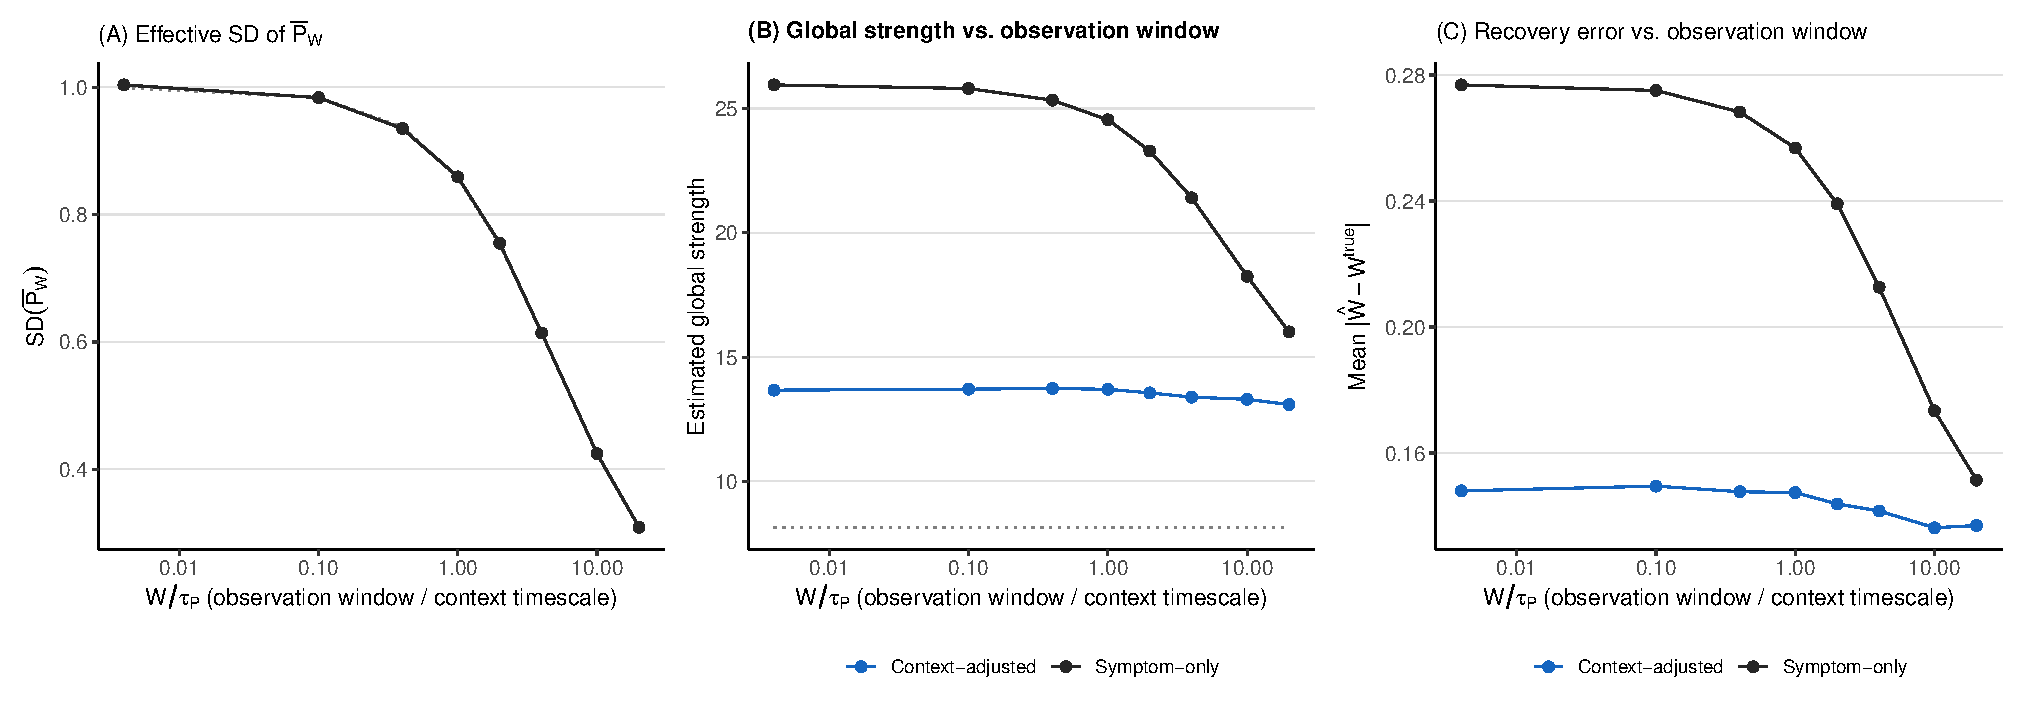
\includegraphics[width=\linewidth]{figs/Figure_S_network_window_check.pdf}
  \caption{\textbf{Observation-window sensitivity check.} Each simulated person's
  slow-context value was generated as the time-average, $\bar P_W$, of an
  Ornstein-Uhlenbeck process with autocorrelation time $\tau_P = 1/\kappa$, and the
  observation window $W$ was varied on a log scale relative to $\tau_P$.
  \textbf{(A)} Effective between-person standard deviation of $\bar P_W$ (solid) against
  the analytic Ornstein-Uhlenbeck prediction (dotted). \textbf{(B)} Estimated global
  strength for the symptom-only and context-adjusted estimators; the true global strength
  is shown as a dotted reference line. \textbf{(C)} Mean absolute recovery error relative
  to $W^{\mathrm{true}}$ for both estimators.}
  \label{fig:network_window_check}
\end{figure}
